\documentclass[10pt,twocolumn]{extarticle}

\usepackage[margin=0.55in,columnsep=0.22in]{geometry}
\usepackage[T1]{fontenc}
\usepackage{lmodern}
\usepackage{microtype}
\usepackage{booktabs}
\usepackage{tabularx}
\usepackage{array}
\usepackage{graphicx}
\usepackage{xcolor}
\usepackage{enumitem}
\usepackage[font=footnotesize,labelfont=bf]{caption}
\usepackage{titlesec}
\usepackage[most]{tcolorbox}
\usepackage{hyperref}
\usepackage{flushend}

\hypersetup{colorlinks=true,linkcolor=blue!40!black,citecolor=blue!40!black,
  urlcolor=blue!50!black,
  pdftitle={Consequence-Aware Failure Diagnostics for Learned
            Particle-Reconstruction Representations},
  pdfauthor={Dowling Wong}}
\setlength{\parindent}{0pt}
\setlength{\parskip}{1.0pt}
\setlist{nosep,leftmargin=*,topsep=1pt}
\titlespacing*{\section}{0pt}{3.5pt}{1pt}
\titleformat{\section}{\small\bfseries}{\thesection}{0.4em}{}
\newcolumntype{Y}{>{\raggedright\arraybackslash}X}

\title{\vspace{-1.55em}\textbf{Consequence-Aware Failure Diagnostics\\[-0.18em]
for Learned Particle-Reconstruction Representations}\\[-0.12em]
\normalsize Collaboration concept note}
\author{Dowling Wong}
\date{12 August 2026}

\begin{document}
\maketitle
\vspace{-1.9em}

\begin{abstract}
A monitor must answer two questions that average reconstruction accuracy does
not: what declared mechanism caused an alarm, and what scientific consequence
followed. We propose a replay-based diagnosis of frozen representations under
controlled interventions. The central contrast separates acquisition-contract
violations from clean rare-subgroup physics; the corresponding mechanisms are
movement along task-relevant versus redundant representation directions and
loss of support in learned neighbourhoods. We test whether alarms attribute
these families and whether their magnitude predicts downstream loss, explicitly
measuring high-alarm/low-consequence and low-alarm/high-consequence cells. The
testbeds are public neutrino-telescope point clouds and controlled waveforms:
a public TIDMAD denoising benchmark plus a simulator in which assumed and
realized noise covariance are known. Layerwise evidence is compared against
input tests, MMD, classifier two-sample tests, embedding distance, uncertainty,
and output-only monitoring at a matched false-alert budget, with abstention on
families the study never declared.
\end{abstract}

\section{Gap and contribution}

Existing shift monitors can detect changes in inputs, outputs, or embeddings,
but a scientific reconstruction pipeline requires two additional distinctions:
whether the change reflects corrupted acquisition or valid but under-supported
physics, and whether the detected change materially degrades a physics result.
We test whether intermediate representations improve this attribution beyond
generic monitoring at the same false-alert budget, while allowing abstention on
ambiguous or unseen failures. The attribution claim is conditional on the
declared simulator and forward model: unknown physics and model
misspecification are not identifiable from a response profile alone and are
routed to abstention.

In waveform reconstruction, structured acquisition noise induces a likelihood
geometry through the inverse covariance: the correct residual weighting is
$\Sigma^{-1}$, and a model evaluated under the wrong weighting can prefer
reconstructions that are worse in the metric the instrument implies.
Architecture and training coverage further determine which physically relevant
distinctions survive into the representation. This study asks whether
violations of these assumptions can be diagnosed after training, and whether a
detected violation is scientifically consequential. The artifact is a
reproducible experiment suite---configurations, adapters, hooks, replay
scripts, and reports---not a maintained software product.

\textbf{Identifiability limit.} Diagonalizing a covariance yields decorrelated
statistical modes, not labeled physical sources: $\Sigma=\Sigma_1+\Sigma_2$
admits infinitely many positive-semidefinite splits, and low-rank factors are
rotation-degenerate. All attribution here is over \emph{declared intervention
families} under a stated simulator. Observing a response profile does not
identify the cause of an unknown real shift, and we make no such claim.

\section{Failure contracts}

Three declared labels, frozen before evaluation.

\textbf{N---acquisition-contract violation.} For this study the closed family
is power-spectral-density (PSD) or covariance change, jitter, drift, spectral
lines, glitches, tails, hit thinning, and channel or module loss. The
measurement violates a declared acquisition condition; no broader N claim is
made.

\textbf{S---training-support shift.} Window or event composition moves toward
physical strata that are sparse under the clean training distribution. The
events themselves are clean and physically valid; only the support has moved.

\textbf{E---evaluation-contract fault.} Wrong units, coordinate ordering,
output semantics, PSD convention, or metric implementation. This is a pipeline
bug, not a distribution shift.

\textbf{N versus S is the scientific core.} E is decided by deterministic
schema and range invariants, so it is reported as a gate result, not as a class
in a classification score. The informative and difficult separation is N from
S. N and S may both move the observed input distribution, so generic
input-shift detection alone cannot distinguish them. Evidence for N comes from
acquisition-quality indicators, paired corruption interventions, or known
violations of the measurement model. S is defined by physically valid,
uncorrupted events that occupy low-density regions of the clean training
support. The scientific problem is therefore not whether the input changed, but
whether the change reflects corrupted measurement or valid but under-supported
physics. That distinction is what matters operationally: discarding S rejects
physically valid events, whereas rejecting N removes measurements that violate
the declared acquisition contract.

\section{Claims}

\textbf{C1---Detection.} At a 1\% false-alert rate on nominal, non-overlapping
windows, the best monitoring signature detects at least 80\% of held-out abrupt
and gradual N/S shifts within five windows, and is non-inferior to the
strongest eligible baseline by a five-point power margin. Delay is primary in
\emph{windows}.

\textbf{C2---Attribution with abstention.} Two endpoint families are
co-primary. The operational family is macro-F1 over $\{$N,S$\}$ on held-out
cases, with N+S mixtures scored by multi-label F1. The mechanism family is
standardized displacement, neighbour retention, subspace principal angle, and
the layerwise sensitivity profile, each normalized by clean within-stratum
dispersion.

A split-conformal nonconformity score~\cite{angelopoulos2021} is used to
\emph{abstain} on cases that do not resemble the declared training families.
Unseen-family detection is evaluated by AUROC, while attribution quality under
abstention is reported through selective risk and macro-F1 as functions of
retained coverage~\cite{geifman2017}. The selective endpoint is risk--coverage
AUC, with N/S macro-F1 at $80\%$ retained coverage reported alongside it.
Detection of the unknown and attribution among the known are thus not scored as
if they were the same quantity.

The paired difference $\Delta\mathrm{F1}$ between the full layerwise and
all-generic arms is reported with a 95\% confidence interval, and read three
ways. A practically meaningful benefit requires the interval to exclude zero
\emph{and} the point estimate to reach $0.10$ macro-F1; equivalence is supported
if the interval lies within a predeclared $\pm0.05$ margin; otherwise the result
is inconclusive. This lets a strong generic baseline produce a meaningful
negative result --- internal hooks may not justify their cost.
A mechanism metric is promoted from development to the frozen confirmatory set
only if it responds monotonically to the positive-control severity and adds
separation beyond the generic arm; otherwise it remains descriptive.

\textbf{C3---Cost.} Ten-percent event sampling plus fixed-size sketches yields
p95 replay-path latency overhead $<10\%$, $\geq10\times$ less representation
storage, and $\leq5$ points of power or F1 loss relative to full capture.

\textbf{C4---Is an alarm informative about scientific consequence?} Let $A$
be the monitor's alarm magnitude and $K$ the
downstream scientific loss for the same intervention cell. High consequence is
$K\geq\kappa_m$, where $\kappa_m$ is a testbed-specific scientific tolerance
frozen before evaluation --- provisionally a 10\% degradation for the waveform
amplitude task, and for angular or clustering metrics a physically meaningful
change in resolution, efficiency, purity, or ARI rather than a generic
percentage.

\begin{center}
\scriptsize
\captionof{table}{C4 alarm--consequence matrix and endpoints.}
\begin{tabularx}{\columnwidth}{@{}p{0.62in}YY@{}}
\toprule
\mbox{} & $K<\kappa_m$ & $K\geq\kappa_m$ \\
\midrule
Low alarm & quiet/benign & missed consequence \\
Strong alarm & harmless alarm & detected consequence \\
\midrule
Endpoints & \multicolumn{2}{Y}{Primary: among strong-alarm cells,
AUROC/AUPRC for $K\geq\kappa_m$ and conditional high-consequence risk; also
the low-alarm/high-consequence rate. Secondary: within-family $\rho(A,K)$ and
the high-alarm/low-consequence rate.} \\
\bottomrule
\end{tabularx}
\label{tab:c4}
\vspace{-0.3em}
\end{center}

The waveform testbed decides this, because the generator supplies both the
assumed $\hat\Sigma$ used by the encoder and the realized $\Sigma$, permitting a
controlled test of whether alarms correspond to degradation in the correct
likelihood-weighted residual. C4 is primary there and secondary on the
point-cloud testbed, where consequence is downstream reconstruction error and
no exact covariance exists. We state that asymmetry rather than implying
symmetric coverage.

\section{Testbeds and monitoring design}

\textbf{Neutrino-telescope point clouds (realism).} One primary public
configuration with a released checkpoint exposing a 128-dimensional pre-head
event representation. Module dropout, hit thinning, and time jitter instantiate
N; S windows use clean low-density strata in energy, topology,
vertex/containment, and multiplicity, estimated from training data only. One
secondary architecture serves as a consistency check. A paired
detector-geometry contrast is the first joint pilot because both views can share
the same latent event and only physically supported acquisition changes; the
arm remains gated on successful event pairing and matching.

\textbf{Waveforms (mechanism; parallel track).} The synthetic arm uses a
noise-aware linear control and a generator that constructs PSD/cross-spectral
density models, samples seeded frequency-domain coefficients with real-signal
symmetry, and adds declared artifacts. The public TIDMAD arm uses a
$\sim0.6$M-parameter two-stage domain transformer and the release's denoising
score, comparing otherwise identical MSE and inverse-PSD-weighted objectives.
This compact transformer is a diagnostic subject, not a foundation model; a
larger pretrained model is only a later gated comparison.

\textbf{Monitoring comparison.} Each window records input-quality summaries,
named-layer moments or sketches, outputs, uncertainty, delayed task metrics,
and calibration. A regularized logistic classifier is fitted with identical
splits to five arms: input only; output/uncertainty; final embedding only; all
generic-monitor outputs; and the full layerwise signature. The fourth is the
honest strong baseline, committed to in advance. Eligible baselines ---
corrected univariate input tests, RBF-MMD~\cite{gretton2012}, a classifier
two-sample test~\cite{lopezpaz2017}, embedding mean/covariance distance, output
tests, uncertainty/entropy --- receive identical windows and false-alert
budgets. Clean miscalibration is a model result, not automatically a software
bug~\cite{guo2017}; latent displacement is normalized by clean within-class
dispersion. Held-out severities, seeds, support strata, mixtures, and one
unseen family prevent perturbation lookup; windows and thresholds are frozen
after development; intervals resample event groups and perturbation seeds
separately; null results require a passed positive control, adequate precision,
and a predeclared equivalence margin.

\begin{figure*}[!t]
  \centering
  \begin{minipage}[b]{0.43\textwidth}
    \centering
    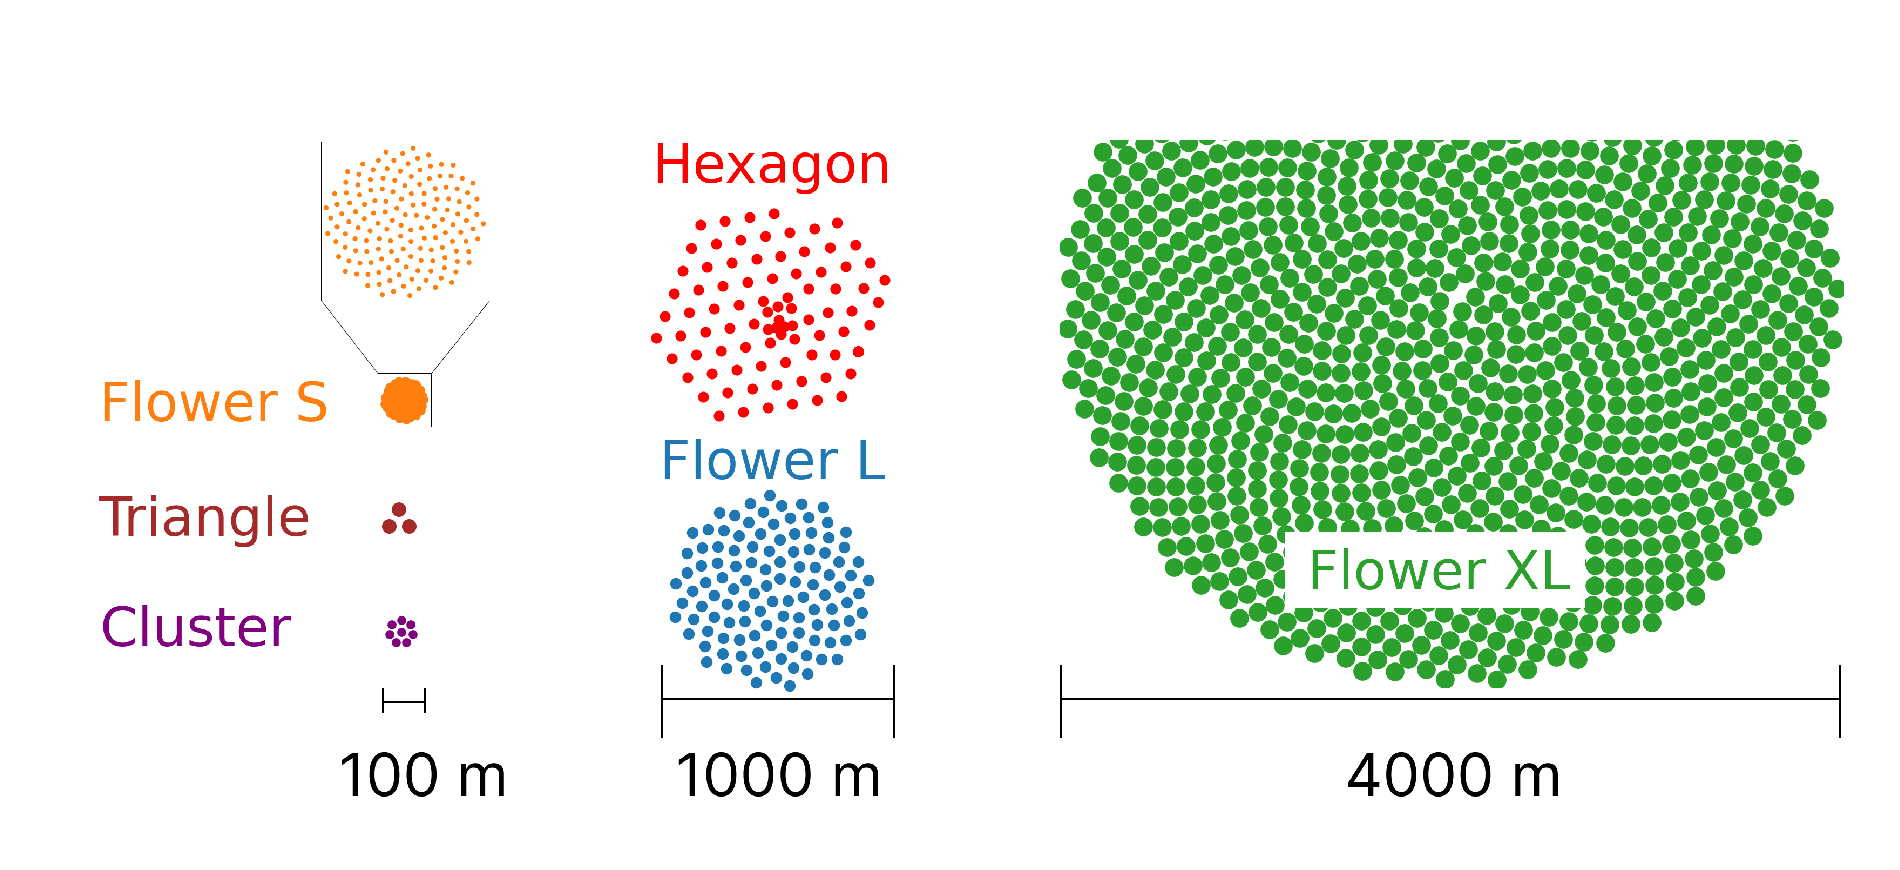
\includegraphics[width=\linewidth,height=0.88in,keepaspectratio]{figures/nubench_detector_geometries.png}\\[-0.2em]
    \scriptsize (a) detector geometries
  \end{minipage}\hfill
  \begin{minipage}[b]{0.25\textwidth}
    \centering
    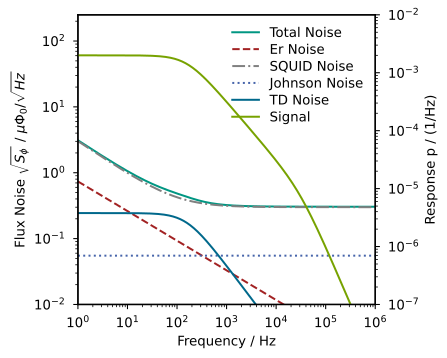
\includegraphics[width=\linewidth,height=0.88in,keepaspectratio]{figures/spectrum_detector_signal_noise.png}\\[-0.2em]
    \scriptsize (b) detector signal/noise spectrum
  \end{minipage}\hfill
  \begin{minipage}[b]{0.28\textwidth}
    \centering
    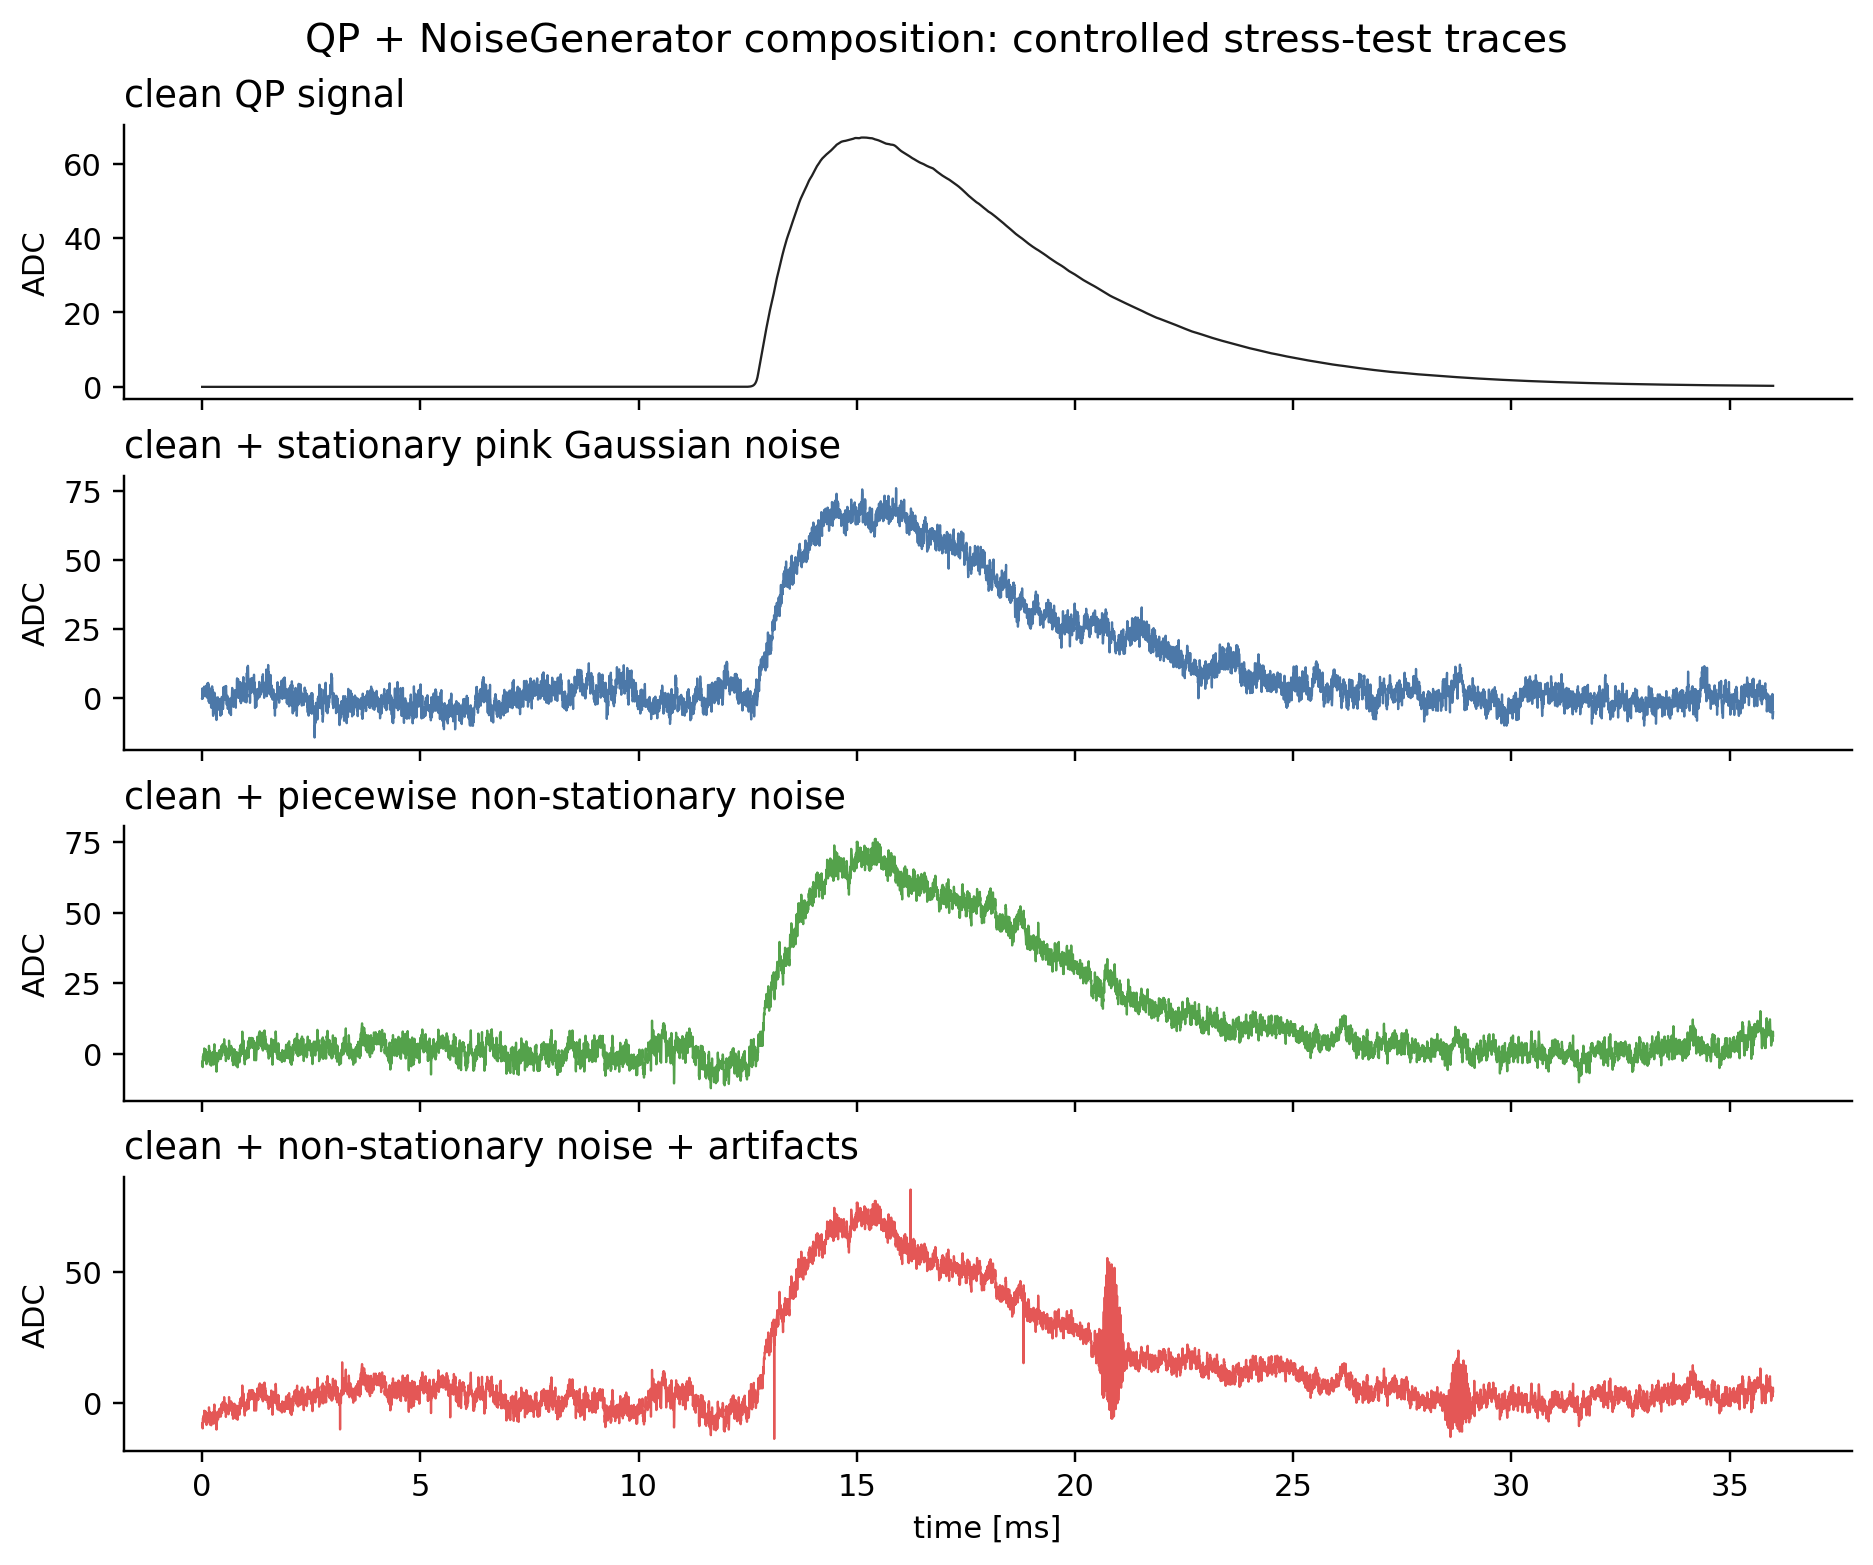
\includegraphics[width=\linewidth,height=0.88in,keepaspectratio]{figures/noise_generator_examples.png}\\[-0.2em]
    \scriptsize (c) generated waveform stress tests
  \end{minipage}
  \vspace{-0.45em}
  \caption{Complementary testbeds. (a) Six top-view geometries, reproduced
  from NuBench Fig.~3~\cite{nubench}. (b) The supplied Al$_2$O$_3$/Al
  athermal-detector response and component PSDs. (c) The generator composes a
  clean optimal-filter-like pulse with stationary colored noise, piecewise
  nonstationarity, and explicit artifacts. Panels (b)--(c) are project outputs.}
  \label{fig:testbeds}
  \vspace{-0.7em}
\end{figure*}

\begin{center}
\scriptsize
\captionof{table}{Core experiment matrix. C1--C3 run on both testbeds; C4 is
primary on waveforms.}
\begin{tabularx}{\columnwidth}{@{}p{0.16in}p{0.95in}Y@{}}
\toprule
ID & Test & Primary endpoints \\
\midrule
E0 & Clean replay; deliberate E faults & Reference discrepancy; gate
sensitivity/specificity \\
E1 & Held-out abrupt/gradual N/S & Power at 1\% false alert; AUROC/AUPRC;
delay in windows \\
E2 & N/S attribution, mixtures, unseen family & Macro/multi-label F1 over
$\{$N,S$\}$; paired CI vs generic arm; unknown AUROC \\
E3 & Capture vs sample/sketch & p50/p95 latency; bytes/event; power/F1 loss \\
E4 & Alarm vs consequence (C4) & $\rho(A,K)$; AUROC for $K\geq\kappa_m$;
off-diagonal rates \\
\bottomrule
\end{tabularx}
\label{tab:experiments}
\vspace{-0.5em}
\end{center}

\section{Staged joint roadmap}

\begin{tcolorbox}[colback=black!3,colframe=black!35,boxrule=0.4pt,
  left=4pt,right=4pt,top=3pt,bottom=3pt,arc=1pt]
\footnotesize
\textbf{Phase 1 (B): paired detector geometry.} Run the first joint pilot on
common latent events under one declared acquisition intervention. Without the
pairing gate, report only a consistency comparison, not a causal layout claim.

\textbf{Phase 2 (A): SPINE/Graph-SPICE transfer.} On one frozen checkpoint,
test one physically justified perturbation and one point-representation metric
against clustering efficiency, purity, fragmentation, or merging near vertices.

\textbf{Phase 3 (A$\oplus$B): target experiment.} If both pilots pass, compare
physics-supported geometry/acquisition interventions with matched non-physical
representation changes at the same displacement magnitude. This is the
unifying attribution test, not an assumption that every learned coordinate is
meaningful.
\end{tcolorbox}

\textbf{Relation to chained-model uncertainty propagation.} Douglas et
al.~\cite{douglas2024} propagate input uncertainty through a chained
neutrino-LAr reconstruction and compare uncertainty-aware and blinded models
under synthetic noise. Here the model is frozen: the question is whether its
representation attributes a declared failure, abstains outside scope, and
links an alarm to consequence. Propagated uncertainty is therefore a candidate
covariate, not the endpoint.

\section{Collaboration}

The agreed sequence is B$\rightarrow$A$\rightarrow$A$\oplus$B, while the
waveform/TIDMAD arm runs in parallel and supplies the first code-complete
contrast. Work should move to a new shared repository rather than debugging the
old inaccessible link. A proposed fortnightly meeting reviews one frozen
protocol or result; initial ownership is waveform infrastructure and generic
monitoring on Dowling's side, and geometry/SPINE physics choices and validation
on Junjie's side, with thresholds and claim changes approved jointly. The first
meeting should freeze one geometry intervention, pairing variables, one
representation endpoint, and one downstream physics endpoint.

\section{Feasibility gate}

Dataset access, checkpoint loading, released-prediction rescoring,
intermediate-hook extraction, and a monotone module-dropout positive control
have been validated ($15.28^\circ\!\to\!25.12^\circ$ median angular error and
10-NN retention $1.000\!\to\!0.393$ across $0$--$50\%$ dropout). Exact
re-inference parity remains unresolved: the current pipeline differs from the
released directions by $0.944^\circ$ median angular error. Exact identity is a
software control, separate from the scientific geometry gate. On a fixed
development subset we will test whether that offset is stable across severity
and event strata. Stable offsets permit a predeclared backend tolerance for the
paired contrast; severity-dependent drift is a confound and keeps the gate
closed.

\begin{thebibliography}{7}
\scriptsize
\setlength{\itemsep}{-1.6pt}\setlength{\parsep}{0pt}
\bibitem{nubench} R.~F. \O rs\o e et al. ``NuBench: An Open Benchmark for Deep
Learning-Based Event Reconstruction in Neutrino Telescopes.'' JINST 21 (2026).
\href{https://arxiv.org/abs/2511.13111}{arXiv:2511.13111}.
\bibitem{koh2020} D.~H. Koh et al. (DeepLearnPhysics). ``Scalable,
Proposal-free Instance Segmentation Network for 3D Pixel Clustering and
Particle Trajectory Reconstruction in LArTPCs.''
\href{https://arxiv.org/abs/2007.03083}{arXiv:2007.03083} (2020).
\bibitem{douglas2024} D. Douglas, A. Mishra, F. Petersen, D. Ratner,
K. Terao. ``Uncertainty Propagation within Chained Models for Machine Learning
Reconstruction of Neutrino-LAr Interactions.''
\href{https://arxiv.org/abs/2411.09864}{arXiv:2411.09864v3}, preprint (2025).
\bibitem{angelopoulos2021} A.~N. Angelopoulos and S. Bates. ``A Gentle
Introduction to Conformal Prediction.''
\href{https://arxiv.org/abs/2107.07511}{arXiv:2107.07511} (2021).
\bibitem{geifman2017} Y. Geifman and R. El-Yaniv. ``Selective Classification
for Deep Neural Networks.'' NeurIPS (2017).
\bibitem{gretton2012} A. Gretton et al. ``A Kernel Two-Sample Test.'' JMLR 13
(2012), 723--773.
\bibitem{lopezpaz2017} D. Lopez-Paz and M. Oquab. ``Revisiting Classifier
Two-Sample Tests.'' ICLR (2017).
\bibitem{guo2017} C. Guo et al. ``On Calibration of Modern Neural Networks.''
ICML (2017).
\end{thebibliography}

\end{document}
